\bgroup
\begin{frame}{Example of greedy action selection}
\begin{minipage}{0.4\textwidth}
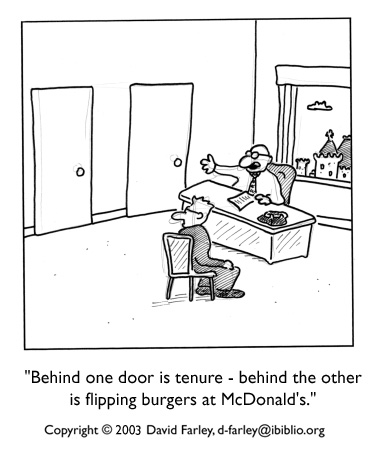
\includegraphics[width=\textwidth]{img/doors.jpg}
\end{minipage}
\begin{minipage}{0.55\textwidth}
\begin{itemize}
\item There are two doors in front of you.
\item You open the left door and get reward 0\\
\textcolor{mImagelabRed}{V(left) = 0}
\item You open the right door and get reward +1\\
\textcolor{mImagelabRed}{V(right) = +1}
\item You open the right door and get reward +3\\
\textcolor{mImagelabRed}{V(right) = +2}
\item You open the right door and get reward +2\\
\textcolor{mImagelabRed}{V(right) = +2}
\begin{equation*}
\vdots
\end{equation*}
\item Are you sure you've chosen the best door?
\end{itemize}
\end{minipage}
\end{frame}
\egroup